\section{Results}
Figure \ref{fig:SearchtimePrefix} shows the measured search times for the prefix search indexes, when finding a prefix.

\begin{figure}[ht!]
    \centering
    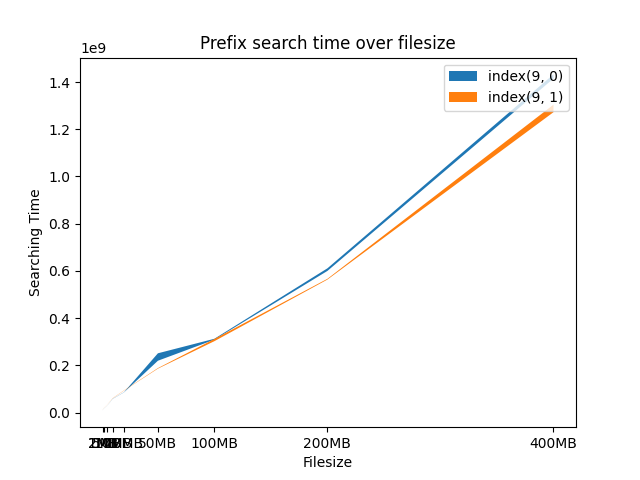
\includegraphics[width=.8\textwidth]{LaTeX/Pictures/Results/Prefixsearch.png}
    \caption{Search times for the prefix search function of Index9.0 and 9.1. Every search query consists of three characters followed by a '*'. The time on the y-axis is measured in $ns$}
    \label{fig:SearchtimePrefix}
\end{figure}

Figure \ref{fig:IndexingBoolPrefi} shows the measured indexing time for the prefix search indexes and the Boolean indexes for comparison.

\begin{figure}[ht!]
    \centering
    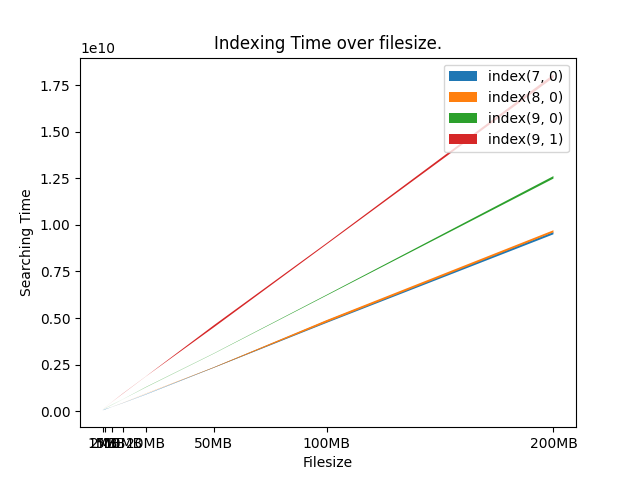
\includegraphics[width=.8\textwidth]{LaTeX/Pictures/Results/Indexing[(7, 0), (8, 0), (9, 0), (9, 1)].png}
    \caption{Indexing times for the prefix search function of Index9.0 and 9.1. The time on the y-axis is measured in $ns$}
    \label{fig:IndexingBoolPrefi}
\end{figure}

